\documentclass[useAMS, usenatbib, preprint, 12pt]{aastex}
\usepackage{cite, natbib}
\usepackage{float}
\usepackage{epsfig}
\usepackage{cases}
\usepackage[section]{placeins}
\usepackage{graphicx, subfigure}
\usepackage{color}
\usepackage{bm}

\bibliographystyle{aasjournal}

\newcommand{\Kepler}{{\it Kepler}}
\newcommand{\kepler}{\Kepler}
\newcommand{\corot}{{\it CoRoT}}
\newcommand{\Ktwo}{{\it K2}}
\newcommand{\ktwo}{\Ktwo}
\newcommand{\TESS}{{\it TESS}}
\newcommand{\LSST}{{\it LSST}}
\newcommand{\Wfirst}{{\it Wfirst}}
\newcommand{\SDSS}{{\it SDSS}}
\newcommand{\PLATO}{{\it PLATO}}
\newcommand{\Gaia}{{\it Gaia}}
\newcommand{\gaia}{{\it Gaia}}
\newcommand{\RAVE}{{\it RAVE}}
\newcommand{\rave}{{\it RAVE}}
\newcommand{\Teff}{$T_{\mathrm{eff}}$}
\newcommand{\teff}{$T_{\mathrm{eff}}$}
\newcommand{\FeH}{[Fe/H]}
\newcommand{\feh}{[Fe/H]}
\newcommand{\ie}{{\it i.e.}}
\newcommand{\eg}{{\it e.g.}}
\newcommand{\logg}{log \emph{g}}
\newcommand{\dnu}{$\Delta \nu$}
\newcommand{\numax}{$\nu_{\mathrm{max}}$}

\newcommand{\racomment}[1]{{\color{red}#1}}

\newcommand{\columbia}{1}
\newcommand{\ww}{2}
\newcommand{\cca}{3}
\newcommand{\florida}{4}
\newcommand{\princeton}{5}
\newcommand{\nsf}{4}
\newcommand{\simons}{2}
\newcommand{\hubble}{7}

\begin{document}

\title{Investigating magnetic dynamo evolution with TESS field dwarfs}

\author{R. Angus\altaffilmark{\columbia}
        J. R. Davenport\altaffilmark{\ww}
        D. Foreman-Mackey\altaffilmark{\cca},
        S. Oh\altaffilmark{\princeton},
        D. Busazi\altaffilmark{\florida},
        A. Mann\altaffilmark{\columbia}
        D. Kipping\altaffilmark{\columbia}
}

\altaffiltext{\columbia}{Department of Astronomy, Columbia University, New
York, NY}
\altaffiltext{\simons}{Simons Fellow, RuthAngus@gmail.com}
\altaffiltext{\ww}{Western Washington University, Bellingham, WA}
\altaffiltext{\nsf}{NSF Fellow}
\altaffiltext{\florida}{Florida Gulf Coast University, Fort Myers, FL}
\altaffiltext{\cca}{Center for Computational Astronomy, Flatiron Institute,
New York, NY}
\altaffiltext{\hubble}{Hubble Fellow}
\altaffiltext{\princeton}{Princeton University, Princeton, NJ}

\section{Introduction}

% Age is a fundamental stellar parameter of great interest to at galactic
% archaeologists and exoplaneteers alike but unfortunately it is a difficult
% attribute to measure for main sequence F, G, K, and M stars in the field.
Of the measurable properties for a large ensemble of field stars, rotation
periods contain the most information about stellar age, and provide the best
leverage for advancing our knowledge of galactic archeology as well as
exoplanet population demographics via gyrochronology.
Angular momentum is carried away though magnetically driven stellar winds,
which slows the star’s rotation over cosmic time.
This rotation-based `clock' is known as gyrochronology.
Cool spots on the star’s surface rotate in-to and out-of view, creating small
amplitude ($\pm$ 1\%) quasi-periodic changes in the stellar brightness.
Using precise light curves available from the \TESS\ mission, we expect to
measure the rotation periods of around ... stars.
Most of these rotation periods will be convertible into ages as they will be
intermediate age FGKM dwarfs.

Some outstanding puzzles regarding the nature of magnetic braking remain to be
answered.
Firstly, a mysterious gap in the rotation period distribution of \Kepler\
dwarfs requires either a sharp transition in magnetic dynamo geometry or a gap
in the local star formation history as an explanation \citep{mcquillan2014,
davenport2017}.
Secondly, a transitioning magnetic dynamo appears to be responsible for
inefficient magnetic braking at old ages in Solar-mass stars.
{\bf We propose to help answer these questions by providing a catalog of \TESS\
rotation periods for all FFI and CTL stars.}
We also intend to use gyrochronology in the cases where it {\it is} applicable
to learn about the evolution of exoplanets and the galaxy as a whole.

\section{Scientific Justification}

The bimodal period distribution among field stars discovered by
\citet{mcquillan2013}, is shown in Figure \ref{fig:davenport}.
Recently, Co-I Davenport discovered this period bimodality extends throughout
all masses in the Kepler rotation sample for nearby stars, as shown in Figure
\ref{fig:davenport} \citep{davenport2017}.
This feature could either reflect a drop in the star formation rate around 600
Myr ago or could be explained by a previously unknown variation in the
spin-down evolution for low-mass stars.
The TESS FFI and CTL targets will provide the ideal dataset to test these two
scenarios explaining the appearance of a period bimodality.
If the bimodal period distribution reflects a age discontinuous age
distribution, the feature should be local; it could
disappear at greater distances or along different lines of sight.
However, if the bimodality is truly due to a transition point in the spin-down
evolution at young ages, there should be little to no variation in the feature
with galactic position.
We will match the TESS FFI and CTL targets to the upcoming data
release from the Gaia mission \citep{perryman2001} to map the rotation period
distribution as a function of galactocentric position.
With the April 2018 data release from Gaia (DR2), we estimate that we will be
able to study rotation periods for G dwarfs in the TESS FFIs out to $\sim$ 3
kpc.


\begin{figure}
\begin{center}
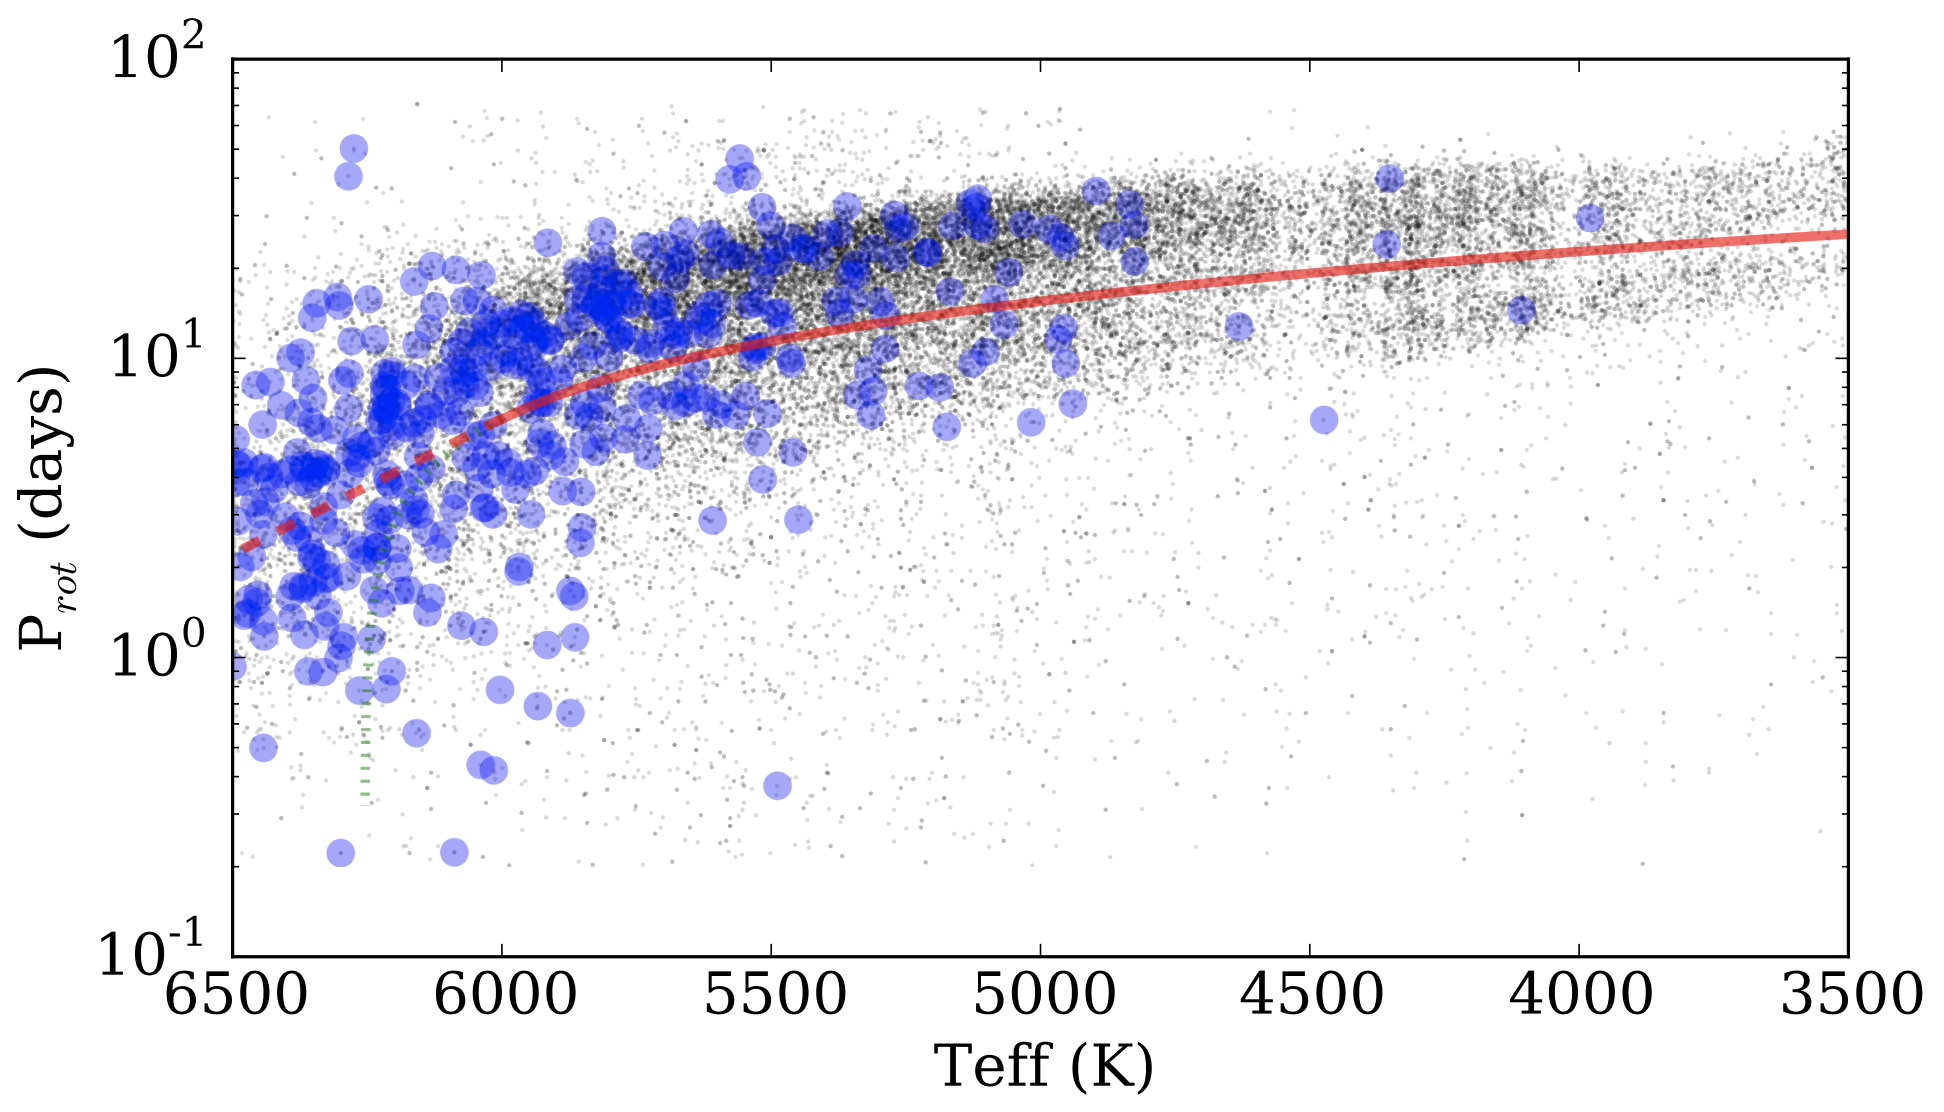
\includegraphics[width=3in, clip=true]{Davenport.png}
\caption{From Davenport (2017).
    Rotation period as a function of effective
temperature for the full McQuillan et al., (2014) Kepler sample in black, and
the subset of these stars that also feature in the TGAS Gaia DR1 catalogue in
blue. Contaminating giants have been removed from the blue sample and the
rotation period bimodality is revealed to exist across all temperatures shown.
    The red line is a 600 Myr rotational isochrone (also known as a gyrochrone).}
\label{fig:davenport}
\end{center}
\end{figure}

Although the classical spin-down law of \citet{skumanich1972}: Period
$\propto$ Age$^1/2$ holds for all open clusters with measured periods, it does
not appear to describe old field stars \citep{angus2015, van-saders2016}.
\citet{van-saders2016} found that including a transition to a weakened magnetic
braking regime in the gyrochronology models, at a critical Rossby number,
provides an improved fit to the data.
Further calibration is needed however; a lack of rotation periods and reliable
ages for old and low-mass stars leaves the rotational evolution of stars older
than the Sun relatively unexplored.
\TESS\ will provide thousands of new rotation periods for both FFI and
two-minute cadence stars, with the maximum measurable period strongly
depending on the length of time it is observed for.
Of particular interest are the, potentially long, rotation periods measurable
for stars that fall in the continuous viewing zones.
Many of these will have spectra from the \TESS\/HERMES survey, from which it
will be possible to calculate isochronal ages, enabling further calibration of
the gyrochronology relations.
We will also use the rotation periods of TESS field dwarfs over the whole sky
to test the gyrochronology relations using galactic kinematics with \Gaia\.
Many stars in the TESS CTL will have proper motions, parallaxes, positions and
radial velocities published in the second \Gaia\ data release.
These parameters provide the information necessary to calculate galactocentric
positions and action angles of the stars, both of which are age indicators.
% PI Angus is currently using the \kepler\ rotation periods of stars in the
% first \Gaia\ data release to calibrate the relations between rotation period
% and vertical action dispersion, two tracers of age.
% Since this relation is likely vary with both galactic longitude and latitude,
% the rotation periods produced from \TESS\ light curves will enable a
% comprehensive, all-sky calibration of these relations.
Since one of the few ways to accurately age-date fully convective, late M
dwarfs is via kinematics, these new relations will help to infer ages for all
stars with M$<$ 0.35M$_\odot$.

In addition, we will use the rotation periods of comoving stars identified in
the first \Gaia\ data release \citep{oh2016} to quantify the accuracy and
precision of gyrochronology.
We have identified 38 stars in 19 pairs with \Gaia\ proper motions and radial
velocities from \RAVE\ that are observable by \TESS, using {\tt tvguide}.
Of these, 34 stars in 17 pairs are already in the CTL list.
Because the stars in these pairs are assumed to be recently disrupted
binaries, we expect them to have the same age and measuring their rotation
periods will therefore allow us to test gyrochronology.

Finally, we hope to use the improved gyrochronology relations, calibrated
using \TESS\ data to infer the dependence of planet frequency on age and
position in the galaxy.
\kepler\ revealed tantalizing hints that exoplanets on short orbital periods
have larger radii and are more infrequent around young stars \citep{mann2017a,
mann2017b, rizzuto2017}.
Do these trends continue into older ages and do they exist in the field?
We will answer these questions by inferring ages for \TESS\ field stars.

% \subsection{The age distribution of exoplanets}

% Of particular interest will be the expected $\sim$ 300 gyrochronal ages of
% exoplanet host stars.
% The gyrochronal ages of these planet hosts, combined with their isochronal and
% kinematic ages may allow us to characterize trends in planet properties over
% time and across the galaxy.
% Additionally, as rotation both influences and is influenced {\it by} stellar
% magnetic fields, it is inextricably related to stellar activity.
% With so many \TESS\ targets being M dwarfs which tend to be particularly
% active, understanding the magnetic behavior of these stars has never been more
% important.

% The ages of \TESS\ stars will also aid galactic archaeology studies,
% traditionally performed with red giants, although greater distances can be
% reached with red giants, main sequence stars are far more numerous.

\section{Technical Feasibility}
The extraction of a rotation period from a light curve can be as simple as
computing a Lomb-Scargle periodogram or, in cases where the signal is less
clear, can be inferred via modeling the correlation between data points.
This latter approach could involve either computing an autocorrelation
function \citep{mcquillan2013}, or fitting a Gaussian process to the time
series \citep{angus2017, foreman-mackey2017}.
In cases where signals have long periods and low amplitudes, care is needed to
separate real astrophysical signal from instrumental systematics.
The measurement of rotation periods is less sensitive to crowding and source
confusion than exoplanet transit characterization because the rotation period
is not effected by photometric dilution.
We will apply two complementary methods to extract and calibrate light curves
from the TESS FFIs.
First, for bright or isolated targets, we will follow \citet{montet2017} to
estimate aperture shapes and perform aperture photometry for bright sources.
Using an ensemble of sources, we will de-trend these light curves using a
modified version of \textsf{everest} \citep{luger2016, luger2017} designed to
preserve photometric signatures of rotation.
This will be achieved by fitting for the systematic effects in the light curve
using the \textsf{everest} model simultaneously with a Gaussian Process model
for the astrophysical variation.
Both \citet{aigrain2016} and \citet{luger2016} demonstrated that this can
preserve stellar variability signals and we will use the \textsf{celerite}
algorithm \citep{dfm2017} to scale the computations to the size of TESS FFI
datasets.
The precision of existing photometric de-trending methods degrades in crowded
fields \citep[for example,][]{luger2017}.
However, to make robust measurements of rotation periods, we do not need
absolutely calibrated light curves.
Therefore, in crowded fields, we will apply a difference imaging method that
was developed for the K2 Campaign 9 microlensing project \citep{henderson2016}
based on the \textsf{CPM} \citep{wang2016} to robustly measure the photometric
variations of crowded sources.
Unlike standard difference imaging methods, this procedure does not require a
reference image.
Instead, a causal data-driven model is built to predict the time series in
every pixel taking systematic effects into account and the residuals between
the observations and the model predictions provide an estimate of the
astrophysical variability in each pixel.
We will tune this method preserve rotation signals and apply it to detect
rotation across the FFIs.

% \begin{figure}
% \begin{center}
% 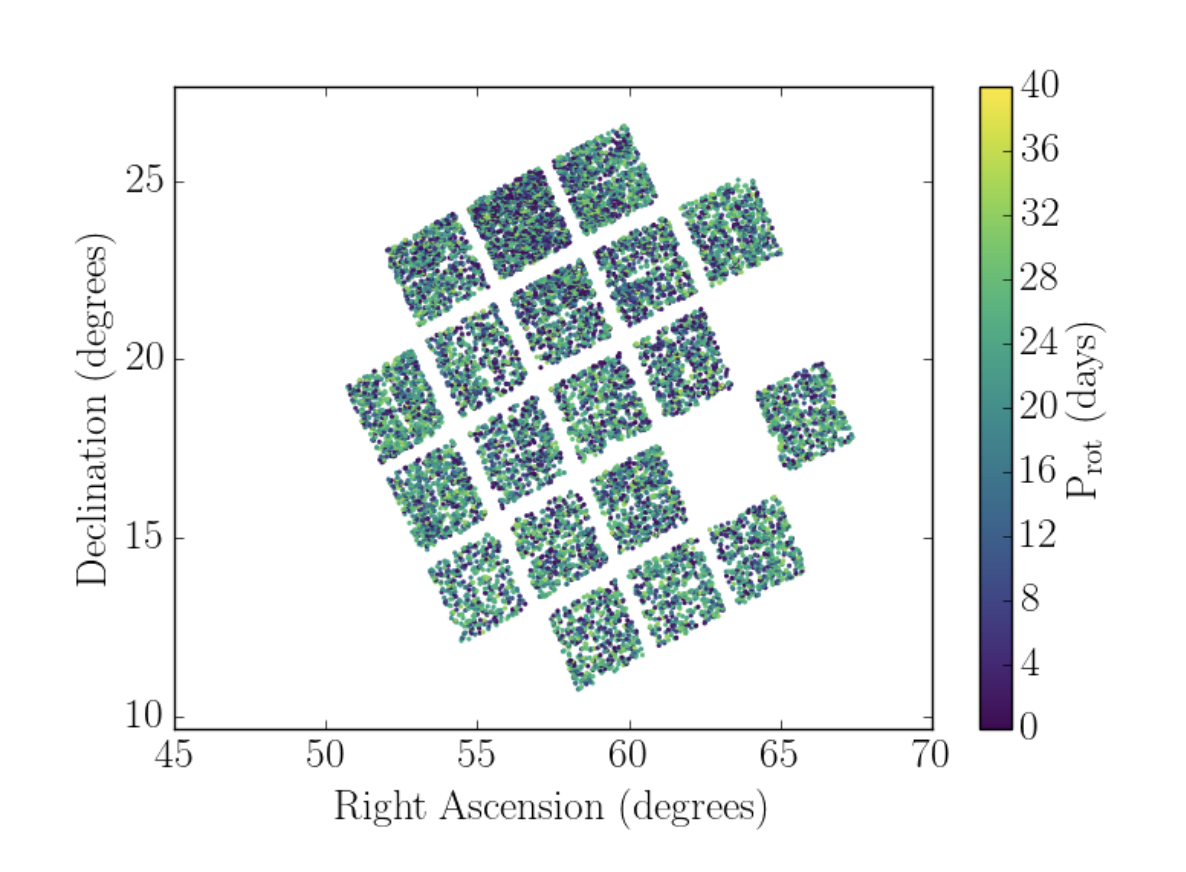
\includegraphics[width=6in, clip=true]{Kalesalad.png}
% \caption{All stars observed during K2 campaign 4, plotted according to their
% equatorial coordinates and colored by their preliminary rotation period.
% These rotation periods were measured using a simple ACF method, applied to
%     everest (Luger et al., 2015) light curves.}
% \label{fig:kalesalad}
% \end{center}
% \end{figure}

\section{Expected Impact}
We will provide light curves and rotation periods for both the two-minute
cadence and FFI targets.

\section{Budget Justification}
PI Angus intends to use the budget to employ a student for 3-4 months.
In this time the student will assist in extracting light curves from the FFIs,
measuring rotation periods and building a rotation period catalog.
The student will also be involved in the scientific project of their choosing:
either the rotation period bimodality, gyrochronology of low-mass stars, or
gyrochronology of comoving pairs.

\bibliography{references}

\end{document}
